%
% kruemmung.tex
%
% (c) 2021 Prof Dr Andreas Müller, OST Ostschweizer Fachhochschule
%
\documentclass[tikz]{standalone}
\usepackage{times}
\usepackage{amsmath}
\usepackage{txfonts}
\usepackage[utf8]{inputenc}
\usepackage{graphics}
\usetikzlibrary{arrows,intersections,math}
\usepackage{ifthen}
\begin{document}

\newboolean{showgrid}
\setboolean{showgrid}{false}
\def\breite{7}
\def\hoehe{9}

\begin{tikzpicture}[>=latex,thick]

% Povray Bild
\begin{scope}
\clip (-6.3,-9.2) rectangle (6.3,7.3);
\node at (0,5.2) {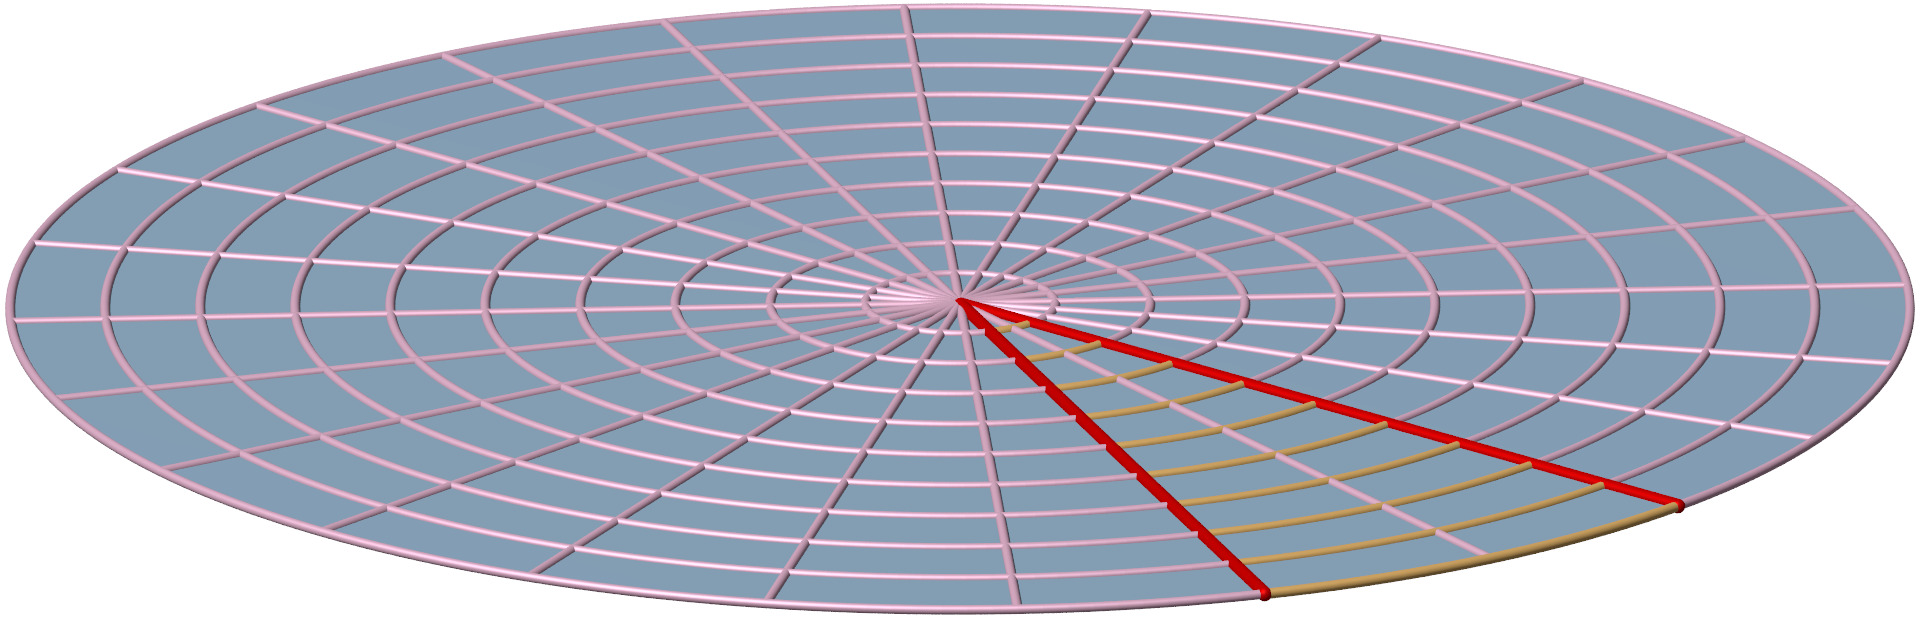
\includegraphics[width=12.6cm]{kruemmung0.jpg}};
\node at (0,0) {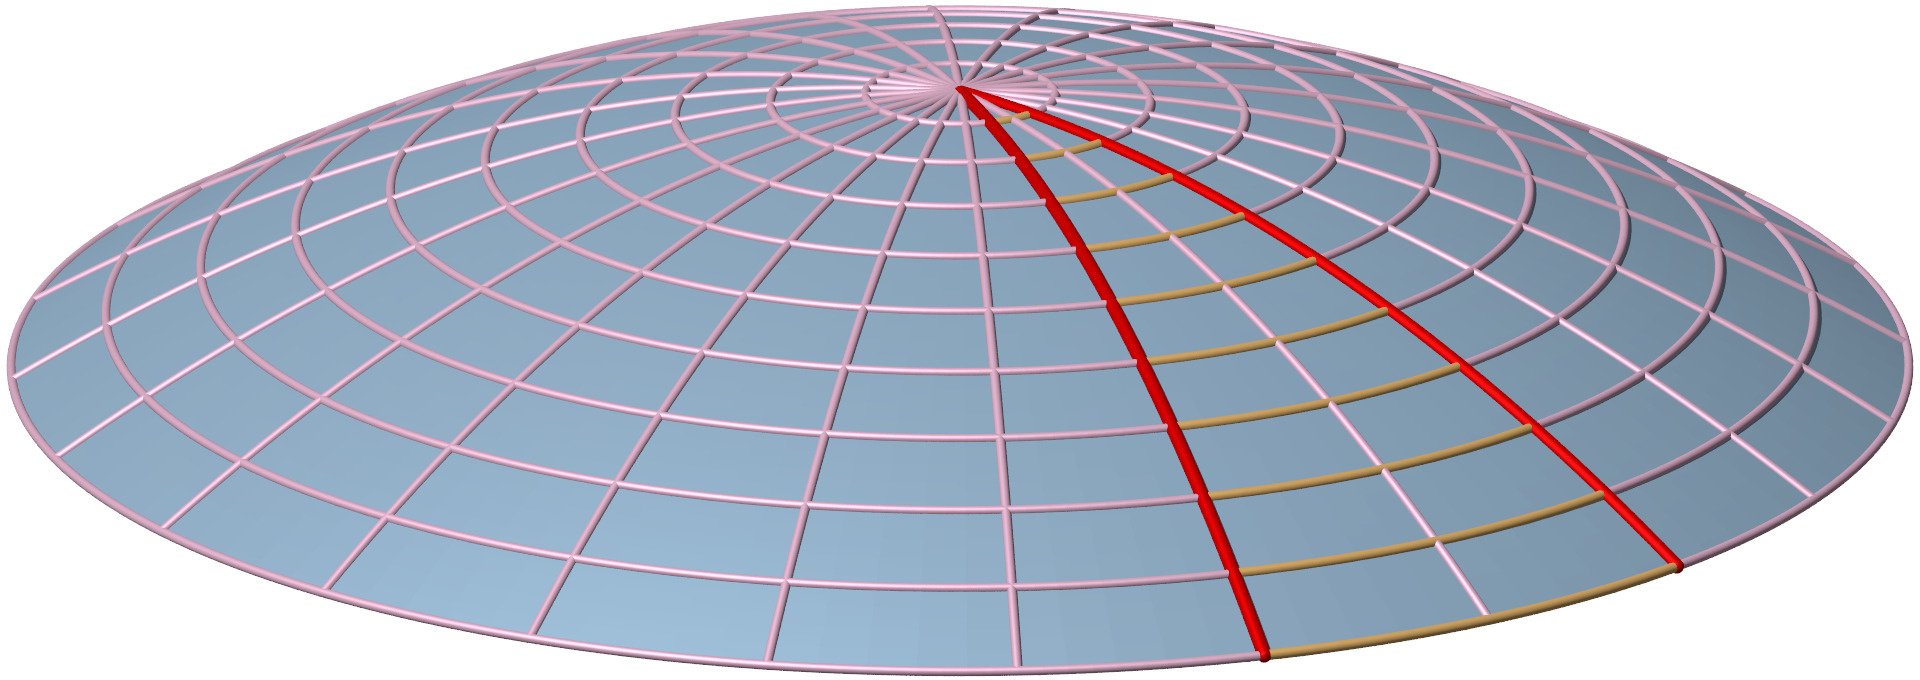
\includegraphics[width=12.6cm]{kruemmungp.jpg}};
\node at (0,-6) {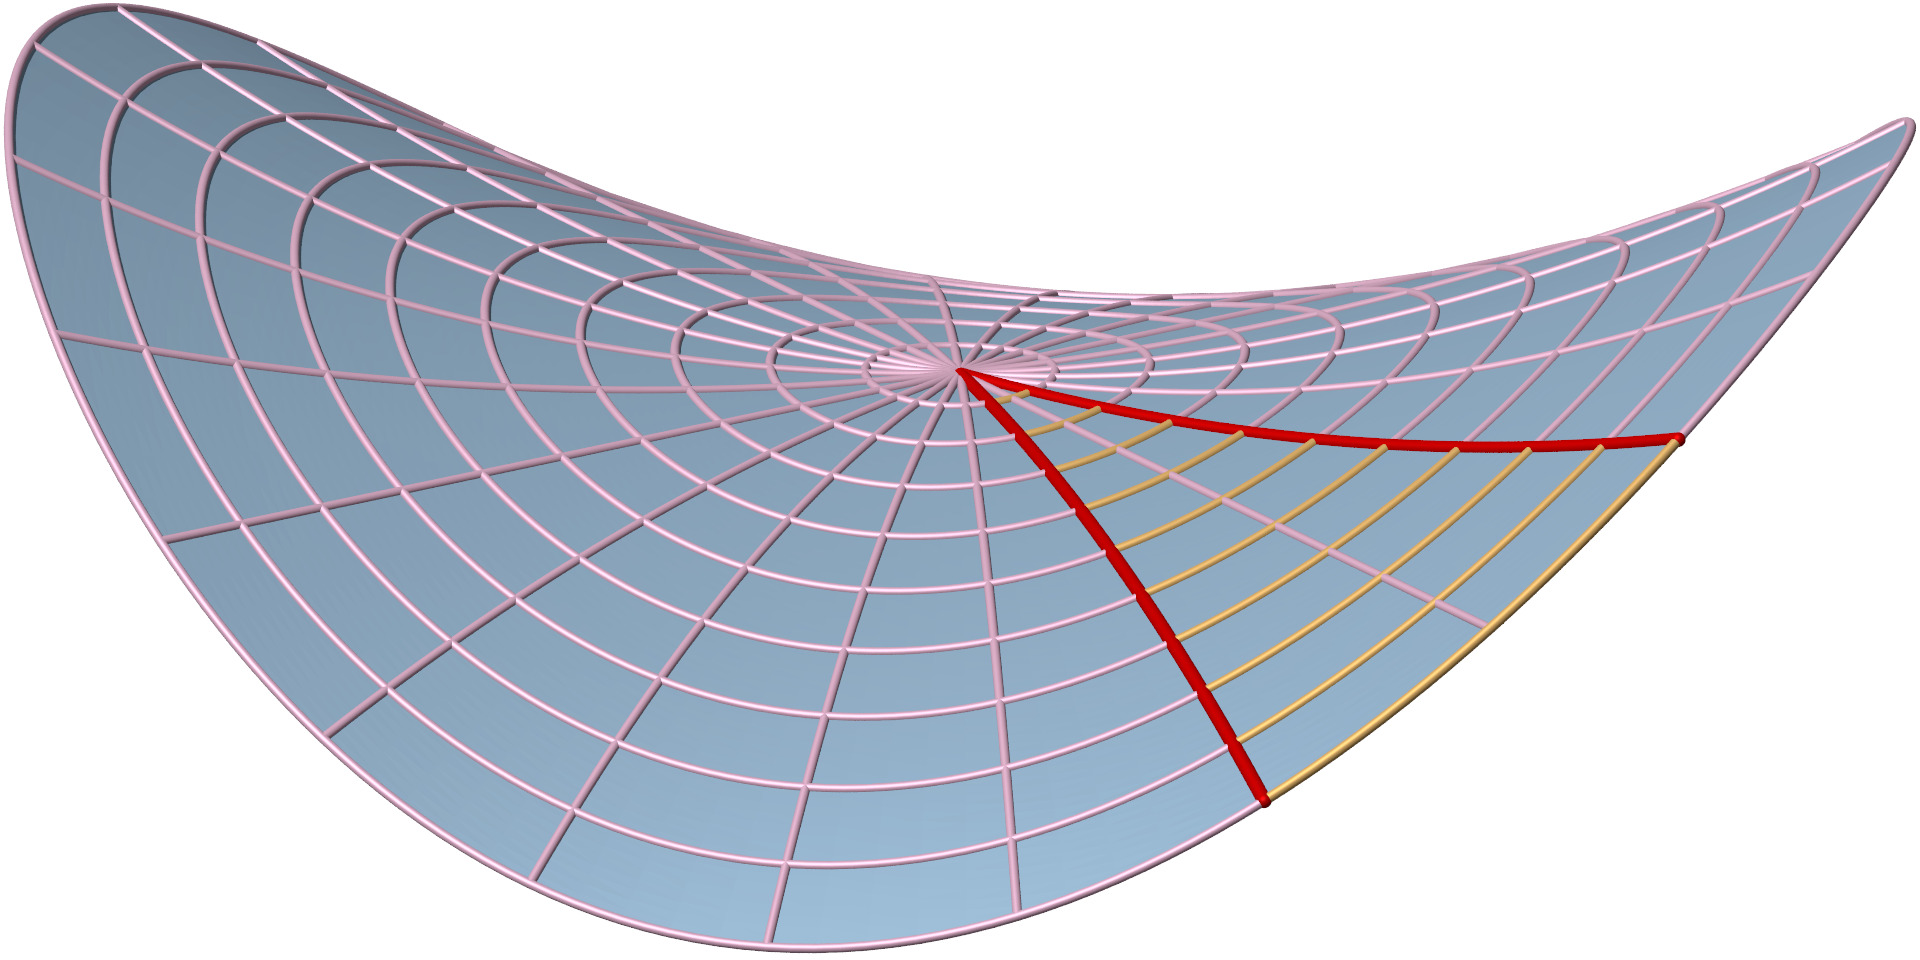
\includegraphics[width=12.6cm]{kruemmungn.jpg}};
\end{scope}

% Gitter
\ifthenelse{\boolean{showgrid}}{
\draw[step=0.1,line width=0.1pt] (-\breite,-\hoehe) grid (\breite, \hoehe);
\draw[step=0.5,line width=0.4pt] (-\breite,-\hoehe) grid (\breite, \hoehe);
\draw                            (-\breite,-\hoehe) grid (\breite, \hoehe);
\fill (0,0) circle[radius=0.05];
}{}

\node at (-6.3,7) [right] {$K=0$};
\node at (-6.3,1.4) [right] {$K>0$};
\node at (-6.3,-7) [right] {$K<0$};

\end{tikzpicture}

\end{document}

